\documentclass{beamer}
\usetheme{default}
\usepackage{lmodern}
\usepackage{amsmath}
\usepackage{amssymb}
\usepackage{proof}
\usepackage{parskip}
\usepackage{wasysym}
\usepackage{hyperref}
\usepackage{verbatim}
\usepackage{relsize}
\usepackage[T1]{fontenc}

\hypersetup{
  colorlinks=true,
  urlcolor=blue
}

\newcommand{\hl}[1]{\color{red}{#1}}
\newcommand{\arr}[1]{\ensuremath\xrightarrow{#1}}

\title{Generating code in a term rewriting framework}
\author{Geoff Hulette}
\date{\today}

\begin{document}

\begin{frame}[plain]
  \titlepage
\end{frame}

%%
\begin{frame}{Outline}

Today I will be talking about:

\begin{enumerate}
  \item Why generating code is difficult
  \item Term rewriting theory
  \item Twig's language
  \item How Twig generates code
  \item Example: generating code for GPUs
\end{enumerate}

\end{frame}


%%
\begin{frame}{Motivation: Proper abstractions}

Writing code is easy when programming abstractions match domain logic. For
example:

\begin{itemize}
\item Matrix calculations in Matlab
\item GUIs in OOP languages
\item Interpreters in ML
\item Device drivers in C
\end{itemize}

The converse also holds; consider any pair-wise permutation in the list above.

\end{frame}


%%
\begin{frame}{Problem: Programming for GPUs}

Writing code for GPUs is tedious. In OpenCL, a simple vector operation
requires more than 200 LOC. 

The abstraction of OpenCL does not match the logic of GPUs.

One solution is to use a higher-level representation for GPU programs, and
generate the low-level CUDA or OpenCL code.

\end{frame}

%%
\begin{frame}{Problem: Programming for GPUs}

Na\"ive GPU code generation may produce inefficient code.

\begin{itemize}

\item We should generate code that supports different data types. Supporting
this capability at runtime may introduce complex conditional branching.

\item We must be careful to avoid copying data to and from the device more
than necessary.

\end{itemize}

\end{frame}


%%
\begin{frame}{Our approach}

To help with this problem, we are working on \textbf{Twig}, a language for
code generation that features:

\begin{itemize}

\item \textbf{Type-directed code generation} to minimize runtime overhead;

\item Simple, user-extensile \textbf{algebraic manipulation} of Twig
expressions, which can eliminate redundant operations.

\end{itemize}

\end{frame}


%%
\begin{frame}{Our approach}

\textbf{Twig}, is based on the theory of \emph{term rewriting}.

In Twig, we use rules that transform \emph{types} in the target language (i.e.
C), and which generate code as a side-effect of application.

\end{frame}


%%
\begin{frame}{Term Rewriting}

\textbf{Term rewriting} is an approach to programming that is well-suited to
code generation. The formalism is based on abstract reduction theory and
universal algebra.

The key idea is to write a program as a set of transformative \emph{rules}
which are applied sequentially to transform inputs to outputs.

\end{frame}


%%
\begin{frame}{Abstract reduction}

\textbf{Reduction} formalizes the idea of step-by-step transformation. An
\textbf{abstract reduction system} is a pair $(A,\to)$ where $\to$ is a binary
relation on $A$.

Some terminology:

\begin{itemize}
  \item $x \in A$ is \textbf{reducible} iff $\exists y \in A$ s.t. $ x \to y$;
  \item $x \in A$ is in \textbf{normal form} if $x$ is not reducible.
\end{itemize}

\end{frame}


%%
\begin{frame}{Equivalence}

If we regard $\to$ as \textbf{identities}, we can ask whether any two objects
in $A$ are \textbf{equivalent}.

\begin{center}
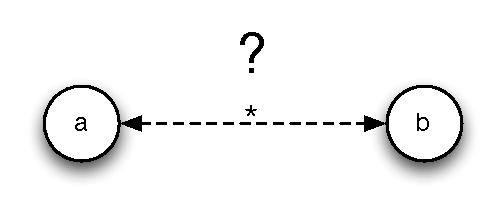
\includegraphics[width=2in]{images/equivalence}
\end{center}

\end{frame}


%%
\begin{frame}{Equivalence}

Deciding equivalence via an undirected search will (probably) be inefficient.

Instead, we can reduce objects to a normal form. If two objects have identical
normal forms, we say they are equivalent.

\begin{center}
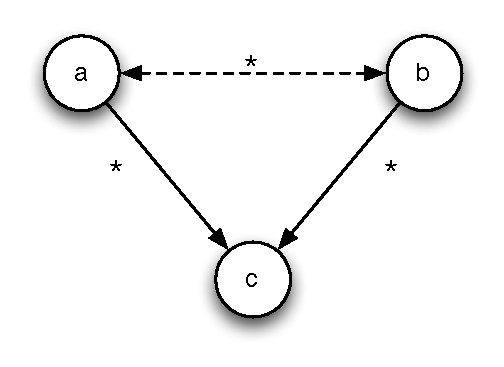
\includegraphics[width=2in]{images/church-rosser}
\end{center}

\end{frame}


%%
\begin{frame}{Equivalence}

Clearly, this approach works iff

\begin{itemize}
  \item reduction eventually \textbf{terminates} and
  \item normal forms are unique, i.e. the system is \textbf{confluent}.
\end{itemize}

\end{frame}


%%
\begin{frame}{Termination}

A reduction system \emph{terminates} iff there exists no infinite chain of
reduction steps, e.g.

\[
a_0 \to a_1 \to a_2 \to \ldots
\]

Naturally, proving termination is undecidable in general.

\end{frame}


%%
\begin{frame}{Confluence}

Every object in a confluent system has at most one normal form. A reduction
system is \emph{confluent} iff

\[
\forall x,y_1,y_2 . 
x \xrightarrow{*} y_1 \land x \xrightarrow{*} y_2 \implies 
\exists z . y_1 \xrightarrow{*} z \land y_2 \xrightarrow{*} z
\]

\begin{center}
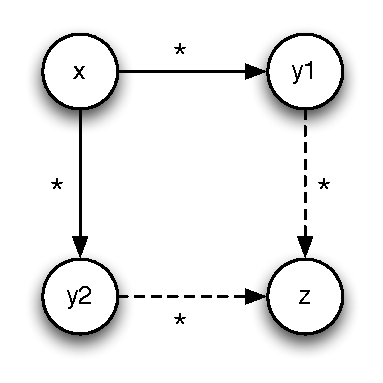
\includegraphics[width=1.5in]{images/confluence}
\end{center}

For a given system $(A,\to)$, confluence is decidable if and only if the
system is terminating.

\end{frame}


%%
\begin{frame}{Confluence and termination}

Note that confluence does not imply termination:

\begin{center}
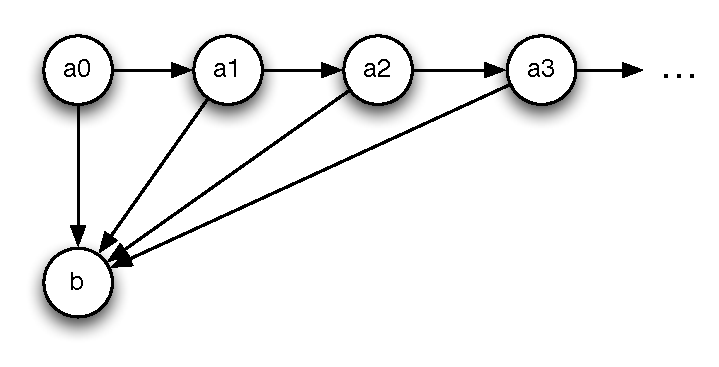
\includegraphics[width=3in]{images/ars}
\end{center}

\end{frame}


%%
\begin{frame}{Terms}

A \emph{term} is tree-structured data with labeled internal nodes, and where
labels represent either \emph{constructors} having 0 or more sub-terms, or
else \emph{variables}.

Terminology:

\begin{itemize}
  \item Constructors with zero arguments are called \emph{constants};
  \item Terms with no variables are called \emph{ground} terms.
\end{itemize}

By (my own) convention, variable names begin with a capital letter, to
distinguish from constructors.

\end{frame}


%%
\begin{frame}{Term example}

The term \texttt{a(b,c(d))} can be represented:

\begin{center}
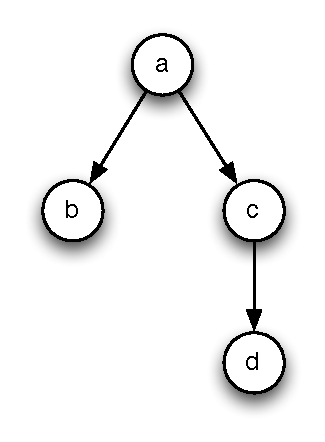
\includegraphics[height=1.5in]{images/example-term-1}
\end{center}

This is a ground term. The functions \texttt{b} and \texttt{d} are constants,
\texttt{c} is unary, and \texttt{a} is binary.

\end{frame}


%%
\begin{frame}{Term example}

The term \texttt{a(X,c(Y,d))} can be represented:

\begin{center}
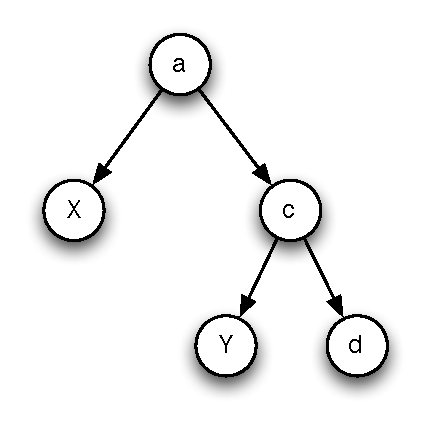
\includegraphics[height=1.5in]{images/example-term-2}
\end{center}

This is not a ground term, and its variables are \texttt{X} and \texttt{Y}.
Note that variables cannot have sub-terms.

\end{frame}


%%
\begin{frame}[fragile]{Matching}

Given a term and a ground term, we can decide if they \emph{match}. If they
do, the match induces an \emph{environment} binding variables to ground terms.

Some examples:

\begin{figure}[h]
\begin{tabular}{|c|c|c|}
\hline
\textbf{Pattern} & \textbf{Input} & \textbf{Result}\\
\hline
\texttt{a(b,c)} & \texttt{a(b,c)} & \{\}\\
\hline
\texttt{a(X,Y)} & \texttt{a(b,c(d,e))} &
  $\{\mathtt{X}=\mathtt{b},\mathtt{Y}=\mathtt{c(d,e)}\}$\\
\hline
\texttt{a(b,c)} & \texttt{a(b,z)} & $\bot$\\
\hline
\end{tabular}
\end{figure}

\end{frame}


%%
\begin{frame}[fragile]{Substitution}

With an environment and a term, we can perform \emph{substitution} to produce
a new ground term.

\begin{figure}[h]
\begin{tabular}{|c|c|c|}
\hline
\textbf{Environment} & \textbf{Term} & \textbf{Result}\\
\hline
$\{\mathtt{X}=\mathtt{b},\mathtt{Y}=\mathtt{c(d,e)}\}$ & 
  \texttt{foo(Y,X)} & \texttt{foo(c(d,e),b)} \\
\hline
$\{\mathtt{X}=\mathtt{b},\mathtt{Y}=\mathtt{c(d,e)}\}$ & 
    \texttt{bar(X,X)} & \texttt{bar(b,b)} \\
\hline
$\{\mathtt{X}=\mathtt{b},\mathtt{Y}=\mathtt{c(d,e)}\}$ & 
    \texttt{Y} & \texttt{c(d,e)} \\
\hline
\end{tabular}
\end{figure}

\end{frame}


%%
\begin{frame}[fragile]{Rules}

We can combine matching and substitution to give a precise definition of a
\emph{rule}.

\begin{center}
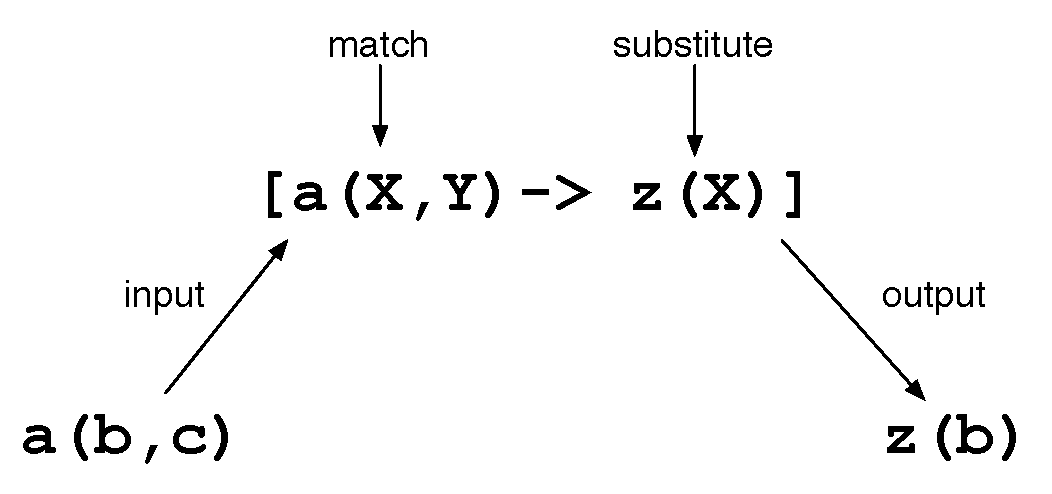
\includegraphics[height=1.5in]{images/rule}
\end{center}

\end{frame}


%%
\begin{frame}[fragile]{Rules}

For example, here are De Morgan's laws:

\begin{itemize}
  \item \texttt{[not(or(P,Q)) -> and(not(P),not(Q))]}
  \item \texttt{[not(and(P,Q)) -> or(not(P),not(Q))]}
\end{itemize}

\end{frame}


%%
\begin{frame}{Twig}

In Twig, we use this term rewriting machinery to define a language for code
generation. Terms represent types in the target language (for now, C), and
rules are transformations between types, i.e. \emph{typemaps}.

\end{frame}


%%
\begin{frame}{Failure}

The result $\bot$ can be interpreted as ``failure'' or ``undefined.'' It is
the result of rule application in case

\begin{itemize}
  \item The input term does not match or
  \item Substitution references undefined variables.
\end{itemize}

\end{frame}


%%
\begin{frame}{Combining rules}

We want to be able to combine rules to build more complex rules. Twig provides
a set of combinators for this purpose.

\end{frame}


%%
\begin{frame}{Twig: Basic combinators}

Sequence:

\[
\infer{t \arr{s_1;s_2} t''}{t \arr{s_1} t' \quad t' \arr{s_2} t''}
\qquad 
\infer{t \arr{s_1;s_2} \bot}{t \arr{s_1} \bot}
\qquad
\infer{t \arr{s_1;s_2} \bot}{t \arr{s_1} t' \quad t' \arr{s_2} \bot}
\]

Left-biased choice:

\[
\infer{t \arr{s_1|s_2} t'}{t \arr{s_1} t'}
\qquad 
\infer{t \arr{s_1|s_2} t'}{t \arr{s_1} \bot \quad t \arr{s_2} t'}
\qquad
\infer{t \arr{s_1|s_2} \bot}{t \arr{s_1} \bot \quad t \arr{s_2} \bot}
\]

\end{frame}


%%
\begin{frame}{System S: More basic combinators}

Constants:

\[
\infer{t \arr{\mathtt{id}} t}{}
\qquad
\infer{t \arr{\mathtt{fail}} \bot}{}
\]

Discard result:

\[
\infer{t \arr{?s} t}{t \arr{s} t'}
\qquad 
\infer{t \arr{?s} \bot}{t \arr{s} \bot}
\qquad
\infer{t \arr{\lnot s} \bot}{t \arr{s} t'}
\qquad 
\infer{t \arr{\lnot s} t}{t \arr{s} \bot}
\]

\end{frame}


%%
\begin{frame}{Properties of Twig's combinators}

A few things to notice about Twig:

\begin{itemize}

\item Rules are applied deterministically, therefore all Twig programs are
confluent.

\item Programs are finite and we do not provide a fix-point combinator,
therefore all Twig programs terminate.

\end{itemize}

\end{frame}


%%
\begin{frame}{Values in Twig}

Types in the target language are values in Twig.

\begin{center}
\begin{tabular}{c | c}
  Twig               & C \\
  \hline                       
  \texttt{int}       & \texttt{int}    \\
  \texttt{double}    & \texttt{double} \\
  \texttt{ptr(int)}  & \texttt{int*}   \\
  \texttt{ptr(char)} & \texttt{char*}  \\
\end{tabular}
\end{center}

\end{frame}


%%
\begin{frame}{Values in Twig}

Twig supports custom mapping between terms and types in the target language,
including application-specific types.

\begin{center}
\begin{tabular}{c | c}
  Twig                  & C \\
  \hline                       
  \texttt{string}       & \texttt{char*} \\
  \texttt{array2D(int)} & \texttt{int**} \\
  \texttt{complex}      & \texttt{struct complex \{double r; double i;\}} \\
\end{tabular}
\end{center}

\end{frame}


%%
\begin{frame}{Extended rules for code generation}

In Twig, code is generated as a side effect of rule evaluation. Primitive
rules can be associated with code \emph{templates}, which are emitted as a
side effect of successful rule application.

We extend the semantics of Twig's combinators to combine templates according
to a formal \emph{template algebra}.

\end{frame}


%%
\begin{frame}{Code templates}

Primitive rules have a syntax for attaching a templates, based on that of
SWIG.

\begin{itemize}
  \item \texttt{[int -> float] \{ \$out = (float)\$in; \}}
  \item \texttt{[string -> int] \{ \$out = atoi(\$in); \}}
\end{itemize}  

Twig takes care of declaring and naming the variables, and supports parameters
and temporary variables.

Twig also has a notion of \emph{tuple} inputs and outputs, but I have elided
this for time.

\end{frame}


%%
\begin{frame}[fragile]{GPU example}

So now we can write our simple GPU example:

\small
\verbatiminput{code/gpu.twig}
\normalsize

\end{frame}


%%
\begin{frame}[fragile]{Algebraic manipulation}

Notice the \texttt{\@reduce} directive:

\begin{verbatim}
@reduce copyArrayFromGPU ; copyArrayToGPU => id
\end{verbatim}

This tells Twig to replace the expression

\texttt{copyArrayFromGPU ; copyArrayToGPU} 

with the identity rule wherever it occurs. The \texttt{@reduce} directive
allows for user-defined algebraic identities.

\end{frame}


%%
\begin{frame}[fragile]{Algebraic manipulation}

Twig provides many built-in identities, for example:

\begin{itemize}
  \item $\mathtt{id;X} \to \mathtt{X}$
  \item $\mathtt{X;fail} \to \mathtt{fail}$
  \item $\mathtt{X;(Y|Z)} \to \mathtt{(X;Y)|(X;Z)}$
  \item $\ldots$
\end{itemize}

These reductions are performed with a general-purpose rewrite engine, so it is
important that the set be confluent and terminating. Twig \textbf{does not}
enforce this!

\end{frame}


%%
\begin{frame}[fragile]{Summary}

\ldots

\end{frame}


%% 
\begin{frame}{Conclusion}

Questions?

My email: \texttt{ghulett@sandia.gov}

\end{frame}


\end{document}
